\documentclass[onecolumn]{article}
%\usepackage{url}
%\usepackage{algorithmic}
\usepackage[a4paper]{geometry}
\usepackage{datetime}
\usepackage[margin=2em, font=small,labelfont=it]{caption}
\usepackage{graphicx}
\usepackage{mathpazo} % use palatino
\usepackage[scaled]{helvet} % helvetica
\usepackage{microtype}
\usepackage{amsmath}
\usepackage{subfigure}
% Letterspacing macros
\newcommand{\spacecaps}[1]{\textls[200]{\MakeUppercase{#1}}}
\newcommand{\spacesc}[1]{\textls[50]{\textsc{\MakeLowercase{#1}}}}

\title{\spacecaps{Assignment Report 1: Process and Thread Implementation}\\ \normalsize \spacesc{CENG2034, Operating Systems} }

\author{Emre Ertürk\\emreerturk3@posta.mu.edu.tr\\https://github.com/Emre81}
%\date{\today\\\currenttime}
\date{\today}

\begin{document}
\maketitle

\begin{abstract}
This homework's goal is to understand child and parent relationships and using multiprocessing method. I used some essential libraries in my python script. I used them for download images, compare image's hash codes, using thread and multiprocessing methods. And I realized python is very suitable language for doing efficient projects.
\end{abstract}


\section{Introduction}
This homework's purpose create a child process and execute some functions in parent process and in child process. In first part, i created a new child process. And I printed the PID of child process's. In the child process i downloaded the images in given array. For the orphan sitution i called a syscall function. I checked images duplicate or not, with using multiprocessing techniques.

\section{Assignments}
I had 4 tasks to do in this homework. I write my script in python language. I used Linux Ubuntu in my virtual machine.

\subsection{Create a child process (os.fork())}

In the tasks one i created a child process and i used os.fork() syscall for it. I printed its pid using os.getpid()
method. As seen in figure 1 parent and child processes have different process ids.

\begin{figure}[h]
\begin{tabular}{ll}
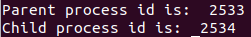
\includegraphics[scale=1]{images/pid2.png}
&
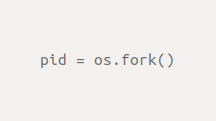
\includegraphics[scale=0.4]{images/fork().png}
\end{tabular}
\caption{Left: Child and Process id. 
Right: usage of os.fork()}
\label{Fig:Race}
\end{figure}

\subsection{Making operations with child process (if (pid == 0))}

In the task two, i downloaded images from the given array under the child process. As seen in Figure 1's right side. I assigned os.fork() method to the pid variable. If pid variable is equals to 0 that means you are in the child process. If pid is greater than 0 that means you are in parent process. I wrote a image downloader function using shutil and requests libraries.The Function gets file name and url as parameters. You can see the image download function in the child process below.

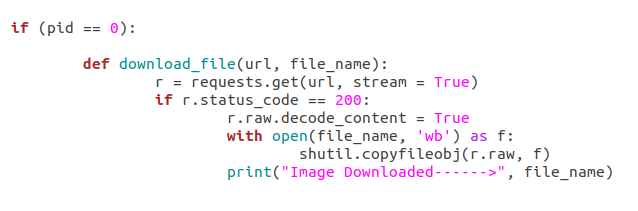
\includegraphics[width=\textwidth]{images/imagedownloader.png}

\subsection{Orphan process (os.wait())}

Orphan process is the situation when the parent finishes before child. I used os.wait() method in the parent process. Parent process waits until child process done. 

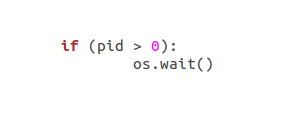
\includegraphics[width=\textwidth]{images/wait.png}

\subsection{Multiprocessing and duplicate file finder (import multiprocessing)}

I searched for a directory and got hash codes of files. I added hash codes to an array and in the for loops, i looked hash codes are duplicate or not. My duplicate finder function gets directory as parameter. So i used globl library and assigned directories to variables. At the last part i called function using multiprocessing, thread and normal technique.

\begin{figure}[ht]
\begin{subfigure}{\textwidth}
  \centering
  % include first image
  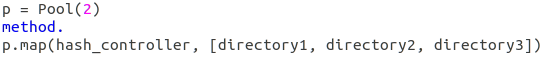
\includegraphics[width=.8\linewidth]{images/poolmethod.png}  
  \caption{Multiprocessing pool method}
  \label{fig:sub-first}
\end{subfigure}
\begin{subfigure}{\textwidth}
  \centering
  % include first image
  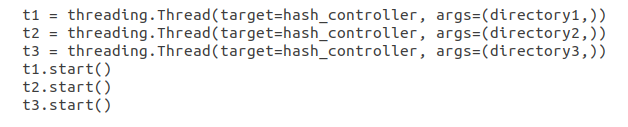
\includegraphics[width=.8\linewidth]{images/thread.png}  
  \caption{Threading method}
  \label{fig:sub-second}
\end{subfigure}
\begin{subfigure}{\textwidth}
  \centering
  % include first image
  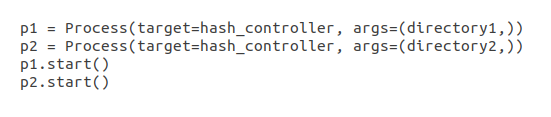
\includegraphics[width=.8\linewidth]{images/process.png}  
  \caption{Process method}
  \label{fig:sub-third}
\end{subfigure}

\caption{As you see 3 different method }
\label{fig:fig}
\end{figure}


\section{Results}

I created child process in task 1. Child process has different process id from parent process.  

\begin{figure}[h!]
  \begin{center}
  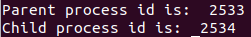
\includegraphics[width=0.5\textwidth]{images/pid2.png}
  \end{center}
  \caption{Parent process id and child process id are different.}
\end{figure}

I used 4 different method to run the duplicate finder function. The most logical method according to the results I got, that is pool method. It is the the most fastest method i tried for this question. Pool method get parameter in array and take elements from array and execute them.




\begin{figure}[h!]
  \begin{center}
  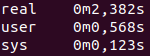
\includegraphics[width=0.5\textwidth]{images/pooltime.png}
  \end{center}
  \caption{Multiprocessing pool method function time.}
\end{figure}

\begin{figure}[h!]
  \begin{center}
  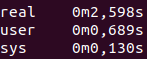
\includegraphics[width=0.5\textwidth]{images/processtime.png}
  \end{center}
  \caption{Multiprocessing process method function time.}
\end{figure}

\begin{figure}[h!]
  \begin{center}
  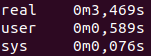
\includegraphics[width=0.5\textwidth]{images/normal.png}
  \end{center}
  \caption{Normal usage of function.}
\end{figure}

\begin{figure}[h!]
  \begin{center}
  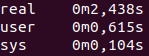
\includegraphics[width=0.5\textwidth]{images/threadingg.png}
  \end{center}
  \caption{Threading method.}
\end{figure}





\section{Conclusion}
    
    We can create child process using os.fork(). We can make different works in parent process and child process, it depends value of os.fork(). os.wait() prevent the orpan sitution. We can run the function with using different techniques. Multiprocessing pool technique was the most efficient method for my function.




\nocite{*}
\bibliographystyle{plain}
\bibliography{references}
\end{document}

